\documentclass{article}
\usepackage[super]{nth}
\usepackage{listings}
\usepackage{graphicx}
\graphicspath{ {images/} }
\lstset{
    numbers=left,
    breaklines=true
    tabsize=2
}
\title{Battleship AI: documentation}
\author{Vardhan Gupta}
\date{may-june 2017}
\begin{document}
   \maketitle
   \tableofcontents
   \section{Introduction}
   This project aims to make an AI which can play the Battleship game intelligently. the code for this is written in python and we aim to use the pygame library of python to implement the graphical part of the game. We also try to look into various algorithms to play the game and finish it efficiently.
   
   \section{the battleship game}
   Battleship is a board game played between two players. each player is supposed to place ships in two different oceans i.e 10x10 grids. the ships are of different sizes namely, aircraft carrier (5x1), battleship (4x1), destroyer (3x1), cruiser (3x1) and a patrol boat (2x1). they may be placed anywhere on the grids either horizontally or vertically. they may never overlap with each other but can be placed adjacent to each other.The players take turns alternatively. On each turn a player is supposed to fire (guess a point on opponent's grid) at the opponents ships which may result in either a 'miss' or a 'hit'. when all the points of a ship have been hit, it results in sinking of that ship. the first player to sink all of opponent's ships is declared the winner.
   
   \section{The project}
   
   \subsection{algorithm 1}
   the algorithm used here is called hunt/target with parity. in this algorithm, it first randomly shoots in a checker board like pattern till a hit is found. once a hit has been found it tries to sink that ship on which the hit was found. if there are no hits left then and everthing is either in 'sink' state or 'miss' state or 'unguessed' state then it goes back to the random shooting.
   
   Once a hit is found, the direction with most unguessed points is chosen to shoot at.


	the functions made so far are:
	\begin{itemize}
   		
   		\item placeship, places ships on the board.
   		\item checksink, checks the sinking status of any ship after a hit.
   		\item shootingdirection, shoots in a given direction in order to sink a ship.
   		\item targetmode, finds the best possible direction to shoot in and recalls itself if a hit is left on the board after sink a ship
	
	\end{itemize}
	
	such an algorithm gave an average of around $56$ moves to beat a random board when tested for $10000$ games.
	
	\subsection{algorithm 2}
	
	the next algorithm used calculates the probability of every unguessed point in the grid having a ship. the point with the best probability is targeted. if multiple points have the maximum probability then a \textit{neighbour score} is calculated for each such point and the point with maximum neighbour score is shot at. if still multiple points qualify, then the point on the checker board like pattern is shot at. if still multiple points qualify, then any one of these points is chosen at random.
	
	Also, after a hit is found, instead of shooting in the direction with most unguessed points, we add the no. of unguessed points of 'up' with 'down' and 'left with 'right' and compare them. the directions which add upto the bigger one of them is chosen and the best direction is now the direction with the most unguessed points of these two.
	
	the functions made/changed for this algorithm are:
	\begin{itemize}
	
		\item calcprob, calculates the probability of having a ship of a particular size over the entire board.
		\item targetmode, changes were made as mentioned above for obtaining better shooting direction after a hit.
		\item nscore, calculates the neighbour score of a given point.
	\end{itemize}
	
	this approach was a significant improvement over the previous one as it resulted in an average of about $44$ moves tested for $10000$ games. This was the result with a random placement of opponent's ships on each game, subject to the constraints of the game and an intelligent placement might result in a worse average.
	
	\subsubsection{use of statistics of opponent's ship placement}
	
	A 2D matrix (oppstatscore) was created which gave scores to corresponding points where a ship was found on the opponent's boards. Also, scores were deducted if a miss occured at any point. points where no shots were fired in the duration of the game were given a "benefit of doubt" and partial scores were given to them. the scores were given as follows: 
	\begin{itemize}
		\item +2 on a hit.
		\item -1 on a miss.
		\item +1 on unknown status of that point.
	\end{itemize}		
This was done to counter strategies which directly work against my own offensive strategy. The coefficient of variance of this matrix was used to see if a change in strategy was required or not. if so, the points with highest scores were hit-at first.
	
	
	\subsubsection{intelligent ship placement}
	
	So far, I had only been placing the ships randomly. A better way to place the ships would be to see the points where the opponent shoots early in the game and not place any of the ships at those points. This was done by using a 10x10 matrix with each point on the grid having an initial score of $0$ and as the opponent shoots at the player board the corresponding point on this matrix get an incrementation in score. i.e.\ $100$ for the \nth{1} point, $99$ for the \nth{2}, etc. based on this score, the ships will now be placed on the best possible blocks with lowest score. On competeting with the same algorithm with random placement of ships, It won about $7$ out of every $10$ games. Here are some screenshots of that match:\newline\newline
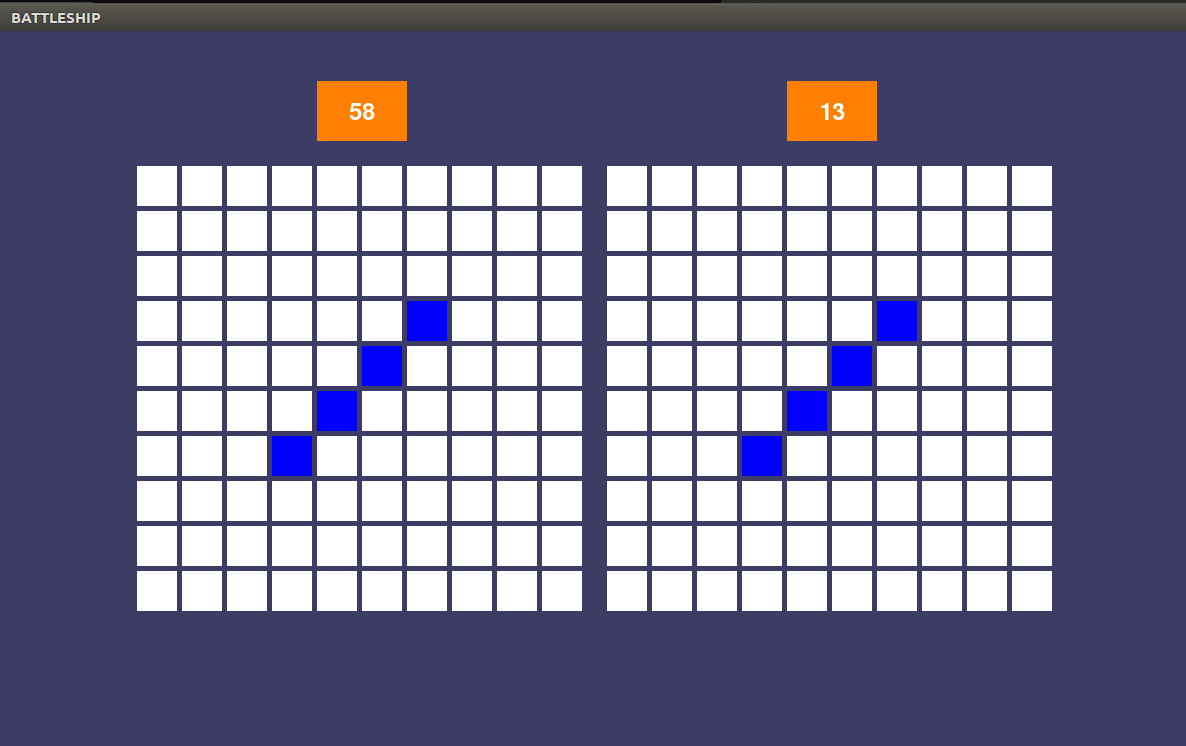
\includegraphics[width=5cm, height=4cm]{shot1}\hspace{2cm}
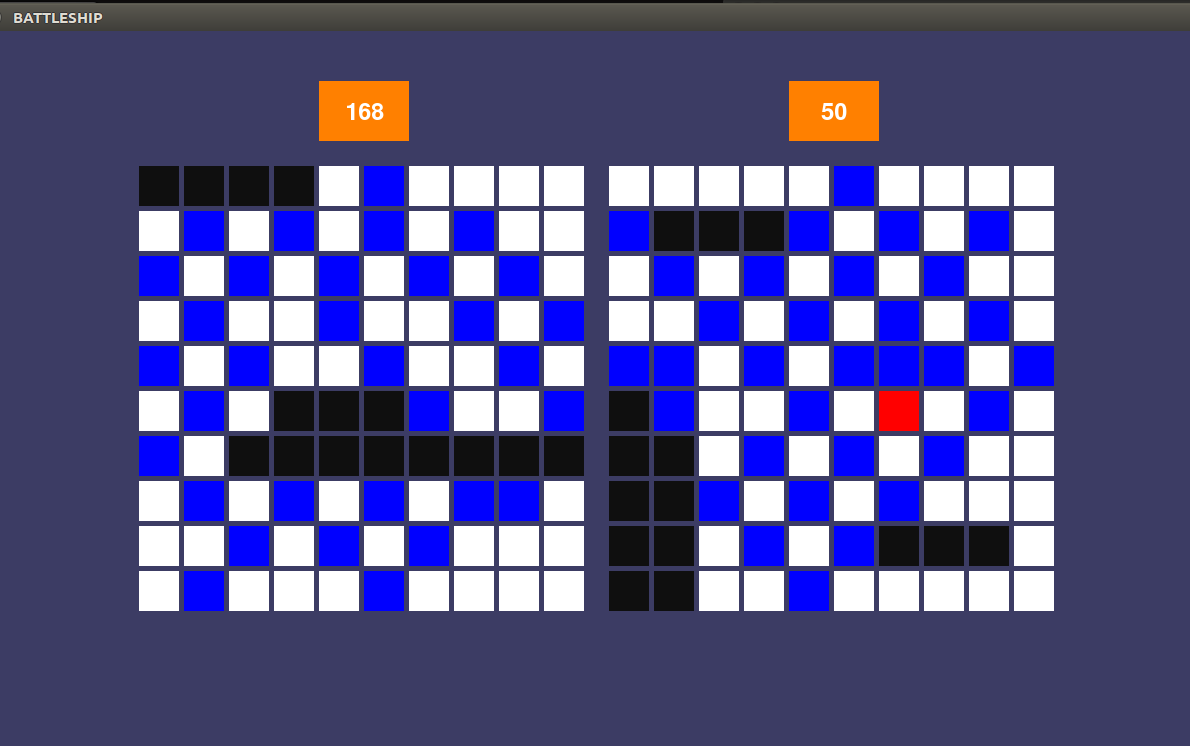
\includegraphics[width=5cm, height=4cm]{shot2}\hspace{2cm}
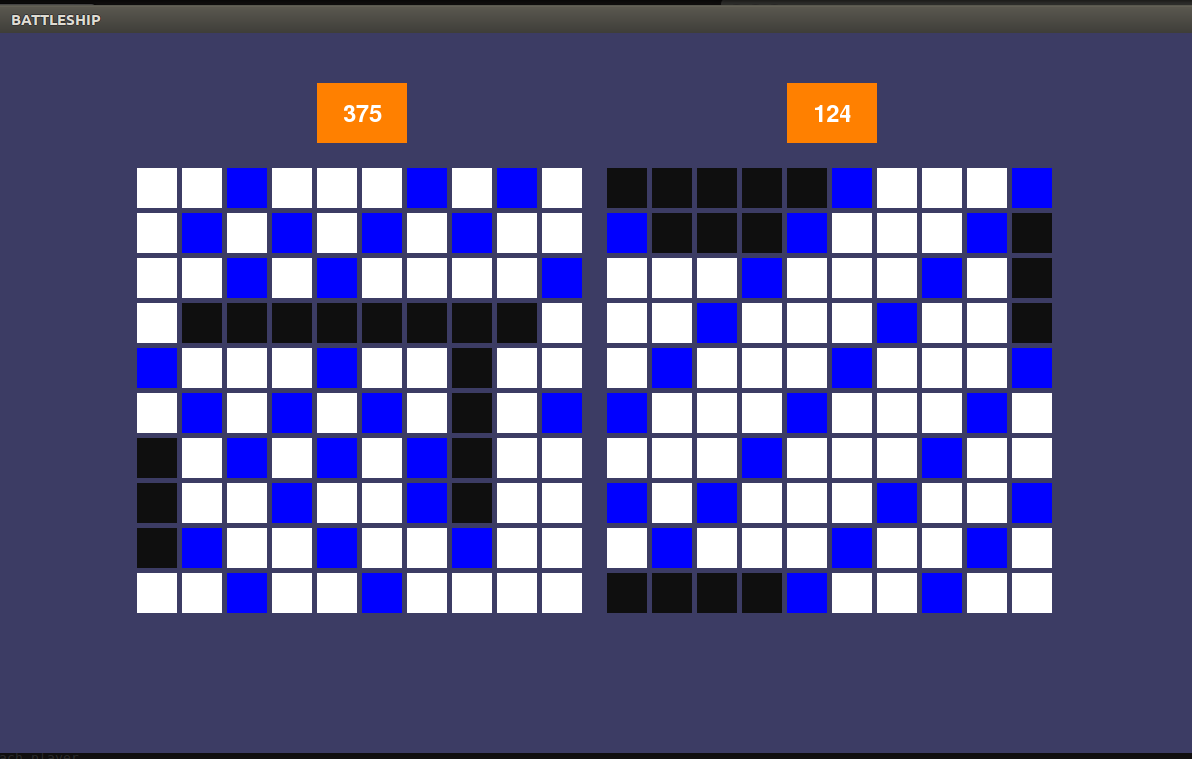
\includegraphics[width=5cm, height=4cm]{shot3}\hspace{2cm}
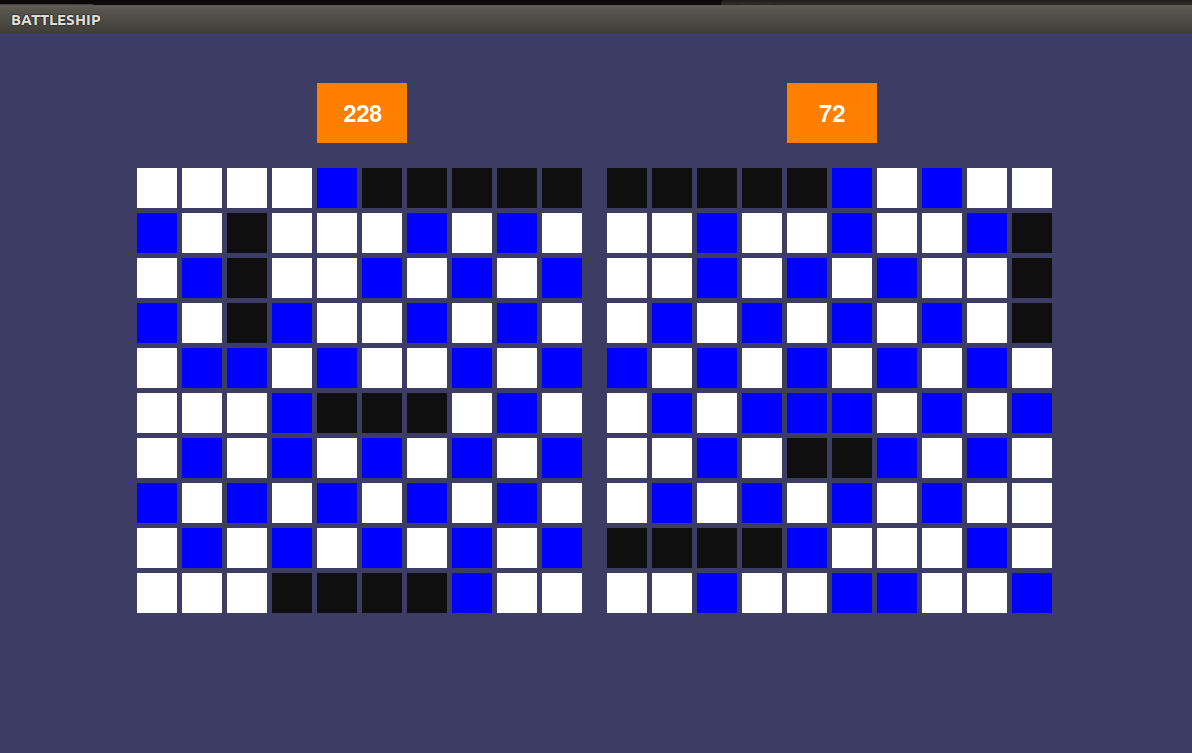
\includegraphics[width=5cm, height=4cm]{shot4}\hspace{2cm}
\newline
Here is the function for calculating the next move on each turn using this algorithm:	
\begin{lstlisting}[language=python,tabsize=2,frame=single,breaklines=true]
def nextmove():
	global checkeredpattern
	maxprob=0
	neighbourscore=[]
	coords=[]
	global bestprob
	for i in range(SIZE):
		for j in range(SIZE):
			if radar[i][j] == unguessed or radar[i][j]==hit:
				for sh in oppships:
					calcprob(i,j,sh) # calculates the no. of ways a ship can be placed on a given point
			if probscore[i][j]==maxprob:
				bestprob.append([i,j]) # the points with maximum probability are placed in bestprob
			elif probscore[i][j]>maxprob:
				bestprob = [[i,j]]
				maxprob = probscore[i][j]
	random.shuffle(bestprob)
	if len(hitfound)==0:	
		if dispersion>0.7 and matchcount>75: #to see if opponent is placing ships in a pattern or not
				coords = bestml()#the best position based on opponent's history
				return coords
		filter2 = []
		bestneighbour=0
		for [i,j] in bestprob:
			neighbourscore.append(findneighbourscore(i,j)) #a subset of bestprob
			if bestneighbour<max(neighbourscore):
				bestneighbour=max(neighbourscore)
				filter2 = [[i,j]]
			elif bestneighbour==max(neighbourscore):
				filter2.append([i,j])
		random.shuffle(filter2)
		coords=random.choice(filter2)
		if (coords[0]+coords[1])%oppships[-1]!=checkeredpattern:
			for [i,j] in filter2:# if still multiple points qualify, points on the checkerboard are preferred
				if (i+j)%oppships[-1]==checkeredpattern:
					coords = [i,j]
					break
	else:#if we have a live hit
		if len(hitfound)==1:#still need to find the orientation of the ship
			coords = random.choice(bestprob)
		else:
			if hitfound[-1][0]==hitfound[0][0]:
				x1=hitfound[0][0]
				y1=probscore[hitfound[0][0]].index(max(probscore[hitfound[0][0]]))
				if probscore[x1][y1]!=0:
					coords = [x1,y1]
				else:
					for [i,j] in bestprob:
						if j==hitfound[0][1]:
							coords=[i,j]
							break
			if hitfound[-1][1]==hitfound[0][1]:
				y1=hitfound[0][1]
				x1=0
				maxx=0
				for i in range(SIZE):
					if maxx<probscore[i][y1]:
						x1=i
						maxx=probscore[i][y1]
				if probscore[x1][y1]!=0:
					coords = [x1,y1]
				else:
					for [i,j] in bestprob:
						if i==hitfound[0][0]:
							coords=[i,j]
							break
						
	if len(coords)==0:#a failsafe if somehow no point is chosen
		coords=random.choice(bestprob)
	cleanprob()
	return coords
\end{lstlisting}

	
	\subsection{the gamemaster file} 
	
	I have also made a file \textit{gamemaster.py} which imports the code of the original file, \textit{battleship.py} and uses it to actually play the game. what this file does is that it will ask a player the coordinates of the point where they want to play their next move. how they choose those particular coordinates is subject to the internal workings of their algorithm. then gamemaster "shoots" at the said coordinates of the opponent's board. the opponent now gives a feedback based on whether the player has missed or hit or sunk a ship. based on this feedback the player will now update their radar. the same process is then repeated with the roles reversed and this continues until someone wins. This file is also where the pygame module is used, to show the games played graphically. The main function of this file is as follows: 
\begin{lstlisting}[language=Python,frame=single,tabsize=2,breaklines=true]
def main():
	global counter,score
	p1.boardgenerator()		#functions to generate boards of each player
	p2.boardgenerator()

	global FPSCLOCK,DISPLAYSURF
	pygame.init()
	BASICFONT = pygame.font.Font('freesansbold.ttf', BASICFONTSIZE) # for writing score
	FPSCLOCK = pygame.time.Clock() # pygame function to run everything at a given FPS
	DISPLAYSURF=pygame.display.set_mode((windowwidth,windowheight)) # generating the window
	
	pygame.display.set_caption('BATTLESHIP') #sets the title
	DISPLAYSURF.fill(bgcolor) 
	abc=0
	noofmoves=0

	while True:		# the main game loop
		noofmoves+=1
		DISPLAYSURF.fill(bgcolor)
		drawRadar(p1.radar,p2.radar,BASICFONT) # for drawing the boards of both players and diplaying the score at a given moment 
		for event in pygame.event.get():
			if event.type == QUIT or (event.type==KEYUP and event.key == K_ESCAPE):
				pygame.quit()
				sys.exit()

		x,y = p1.nextmove()			# nextmove() returns the coordinates(x,y) to shoot at next
		move = p2.hitat(x,y)		# hitat(x,y) returns the feedback on shooting at x,y
		p1.updateradar(x,y,move)	# the feedback from hitat(x,y) is used to update the radar of the player who took the shot
		if len(p1.ships)==0:
# in case of end of a match, all parameters are then reset for each player
			p1.resetplayer(p1)		
			p2.resetplayer(p2)
			score+=1
			counter+=1
			if abc>=matches:
				pygame.quit()
				sys.exit()
			else:
				abc+=1
				noofmoves=0
				p1.boardgenerator()
				p2.boardgenerator()

# the same thing is done again with roles of each player reversed
		x1,y1 = p2.nextmove()
		move1 = p1.hitat(x1,y1)
		p2.updateradar(x1,y1,move1)
		if len(p2.ships)==0:
			p1.resetplayer(p1)
			p2.resetplayer(p2)
			counter+=1
			if abc>=matches:
				pygame.quit()
				sys.exit()
			else:
				abc+=1
				print noofmoves
				noofmoves=0
				p1.boardgenerator()
				p2.boardgenerator()
		
		pygame.display.update()
		FPSCLOCK.tick(FPS)		

\end{lstlisting}
\end{document}
